\documentclass{aip-cp}

\usepackage[numbers]{natbib}
\usepackage{rotating}
\usepackage{graphicx}
\usepackage{url}
\usepackage[utf8]{inputenc}

\begin{document}

\title{gamma-sky.net: Portal to the Gamma-Ray Sky}
\corresp[cor1]{Corresponding author: Arjun.Voruganti@gmail.com}

\author[mpik]{Arjun Voruganti\corref{cor1}}
\author[mpik]{Christoph Deil}
\author[mpik]{Axel Donath}
\author[mpik]{Johannes King}

\affil[mpik]{MPIK, Heidelberg, Germany}


\maketitle

\begin{abstract}
\gammaskyurl is a novel interactive website, created specifically for exploring the gamma-ray sky. The map view is powered by the Aladin Lite sky atlas, which allows interactive pan and zoom navigation as well as search by sky position or object names, similar to Google maps. The initial image shows the gamma-ray sky observed by the Fermi-LAT gamma-ray space telescope, other survey images (e.g. Planck radio image or ROSAT X-ray image) are available for comparison with the gamma-ray data.
Sources from major gamma-ray source catalogs of interest (Fermi-LAT 2FHL, 3FGL as well as a TeV source catalogs) are overlaid as markers. Clicking on a given source shows some information in a popup, and detailed pages for every source are available with details such as source type, literature references, spectra and light-curves.

We want gamma-sky.net to be useful for both professional astronomers as well as the general public. The website was started only very recently. It is being developed as an open-source, open data project on Github (\gammaskygh). We plan to extend it to display more gamma-ray and multi-wavelength data. Feedback and contributions are very welcome!

\end{abstract}

\section{References}

TODO: References that should be mentioned somewhere in the proceeding:

\begin{itemize}
    \item \cite{tevcat} -- TeVCat: An online catalog for Very High Energy Gamma-Ray Astronomy (\url{http://tevcat.uchicago.edu/})
    \item \cite{tgevcat} -- The Very High Energy source catalog at the ASI Science Data Center (\url{http://www.asdc.asi.it/tgevcat/})
    \item \cite{3fgl} -- Fermi Large Area Telescope Third Source Catalog 
    \item \cite{2fhl} -- 2FHL: The Second Catalog of Hard Fermi-LAT Sources
    \item \cite{snrcat} -- A census of high-energy observations of Galactic supernova remnants (\url{http://www.physics.umanitoba.ca/snr/SNRcat/})
    \item \cite{hips} -- Hierarchical progressive surveys (HIPS) (\url{http://aladin.u-strasbg.fr/hips/})
    \item \cite{aladin-lite} -- Aladin Lite: Embed your Sky in the Browser (\url{http://aladin.u-strasbg.fr/AladinLite/})
    \item \cite{gammapy} -- Gammapy - A Python package for gamma-ray astronomy (\url{http://gammapy.org/})
    \item 3FGL interactive table - (\url{http://fermi.gsfc.nasa.gov/ssc/data/access/lat/4yr_catalog/3FGL-table/})
    \item \cite{hgps} -- H.E.S.S. Galactic plane survey (HGPS) -- upcoming TeV maps and catalog we will add.
\end{itemize}


\section{Introduction}

The field of very-high-energy (VHE) astronomy is growing tremendously – while only a decade ago we observed no more than a handful of sources in the GeV range, today we have thousands, including hundreds within the TeV range. This advancement has been made possible due to our novel ground-based Cherenkov telescope instruments. Such systems exhibit more accurate source detections and higher angular resolutions than ever before. Space-based satellites sharing similar technological breakthroughs have further developed the high-energy (HE) range of gamma-ray astronomy, as can be observed in the latest images from the Fermi Large Area Telescope (Fermi-LAT). As a whole, the instruments can capture gamma-rays in a wide spectrum of energies from 10 MeV to 10 TeV. The High Energy Stereoscopic System (H.E.S.S.) Galactic Plane Survey \cite{hgps}, the High-Altitude Water Cherenkov Observatory (HAWC) 1st Year Catalog, and the fourth Fermi-LAT Point Source Catalog (4FGL) are among the highly anticipated surveys that will be unveiled in the near future. Furthermore, with an incoming wave of notable systems planned to operate soon, such as the ground-based Cherenkov Telescope Array (CTA), we expect to discover numerous never-before-seen sources in the gamma-ray sky. With such abundance of HE and VHE sources and a rapid growth of interest in gamma-ray astronomy, there is an increasingly evident need for a central hub of all relevant catalog and image data. Our website (\url{http://gamma-sky.net}) was designed to function as such.

% TODO: make sure these references are put in the appropriate places:
%
% \begin{itemize}
%     \item \cite{tevcat} -- TeVCat: An online catalog for Very High Energy Gamma-Ray Astronomy (\url{http://tevcat.uchicago.edu/})
%     \item \cite{tgevcat} -- The Very High Energy source catalog at the ASI Science Data Center (\url{http://www.asdc.asi.it/tgevcat/})
%     \item \cite{3fgl} -- Fermi Large Area Telescope Third Source Catalog
%     \item \cite{2fhl} -- 2FHL: The Second Catalog of Hard Fermi-LAT Sources
%     \item \cite{snrcat} -- A census of high-energy observations of Galactic supernova remnants (\url{http://www.physics.umanitoba.ca/snr/SNRcat/})
%     \item \cite{hips} -- Hierarchical progressive surveys (HIPS) (\url{http://aladin.u-strasbg.fr/hips/})
%     \item \cite{aladin-lite} -- Aladin Lite: Embed your Sky in the Browser (\url{http://aladin.u-strasbg.fr/AladinLite/})
%     \item 3FGL interactive table - (\url{http://fermi.gsfc.nasa.gov/ssc/data/access/lat/4yr_catalog/3FGL-table/})
%     \item \cite{hgps} -- H.E.S.S. Galactic plane survey (HGPS) -- upcoming TeV maps and catalog we will add.
% \end{itemize}

\section{Idea}

\begin{itemize}

\item Interactive website designed for exploring the gamma-ray sky

\item Survey images of different frequency bands (mainly all-sky) overlaid onto a three-dimensional map. Gamma-ray sources from catalog data are pinpointed onto the map.

\item The website facilitates both quick browsing and deep investigation of sources

\item Understand the context of sources by viewing them on the map

\item Easily compare sources from different catalogs

\item Website targets professional astronomers, but also the general public through
a user-friendly interface and the easily understandable layout of sources plotted over a map.

\item Open source, open data - allows for 1. users to download any data from our website, and 2. for other developers to contribute to the code.

\end{itemize}

\renewcommand{\thefootnote}{\fnsymbol{footnote}}

\section{Features}

The items listed below illustrate the interface of gamma-sky.net and its utilization as a tool for astronomers.

\begin{enumerate}

\item \textbf{Browsing and navigation features} in the Map View component:

\begin{itemize}
\item Pan and zoom
\item Search tools - locate objects by name, association, or coordinate position
\item Toggle and view specific catalog layers and sky images
\item Pop-up information over each source
\item Export and share images from the sky map (in PNG format)
\end{itemize}

\item \textbf{Analysis tools} in the Catalog View component\footnote[1]{Some of the features listed for the Catalog View are currently only available for select catalogs, but they are expected to be a part of all catalogs in the near future.}:

\begin{itemize}

\item Search and select a source by its name
\item Basic information - position, association and class
\item Extension information
\item Spectral index, brightness and flux
\item Distance and redshift
\item Graphs of light curves and emission spectra
\item Detection/observation information - instrument, date of discovery and relevant papers

\end{itemize}

\end{enumerate}

TODO: How does this features list look? Should we make it more ``elegant"/space them out a bit?

\begin{figure}[t]
\centerline{\includegraphics[width=\textwidth]{figures/mapview_wide}}
\caption{Map View.}
\label{fig:mapview}
\end{figure}

\begin{figure}[t]
\centerline{\includegraphics[width=\textwidth]{figures/catview_wide_zoom}}
\caption{Catalog View.}
\label{fig:catview}
\end{figure}

\renewcommand{\thefootnote}{\arabic{footnote}}

\section{Data}

\begin{figure}[tb]
  \centerline{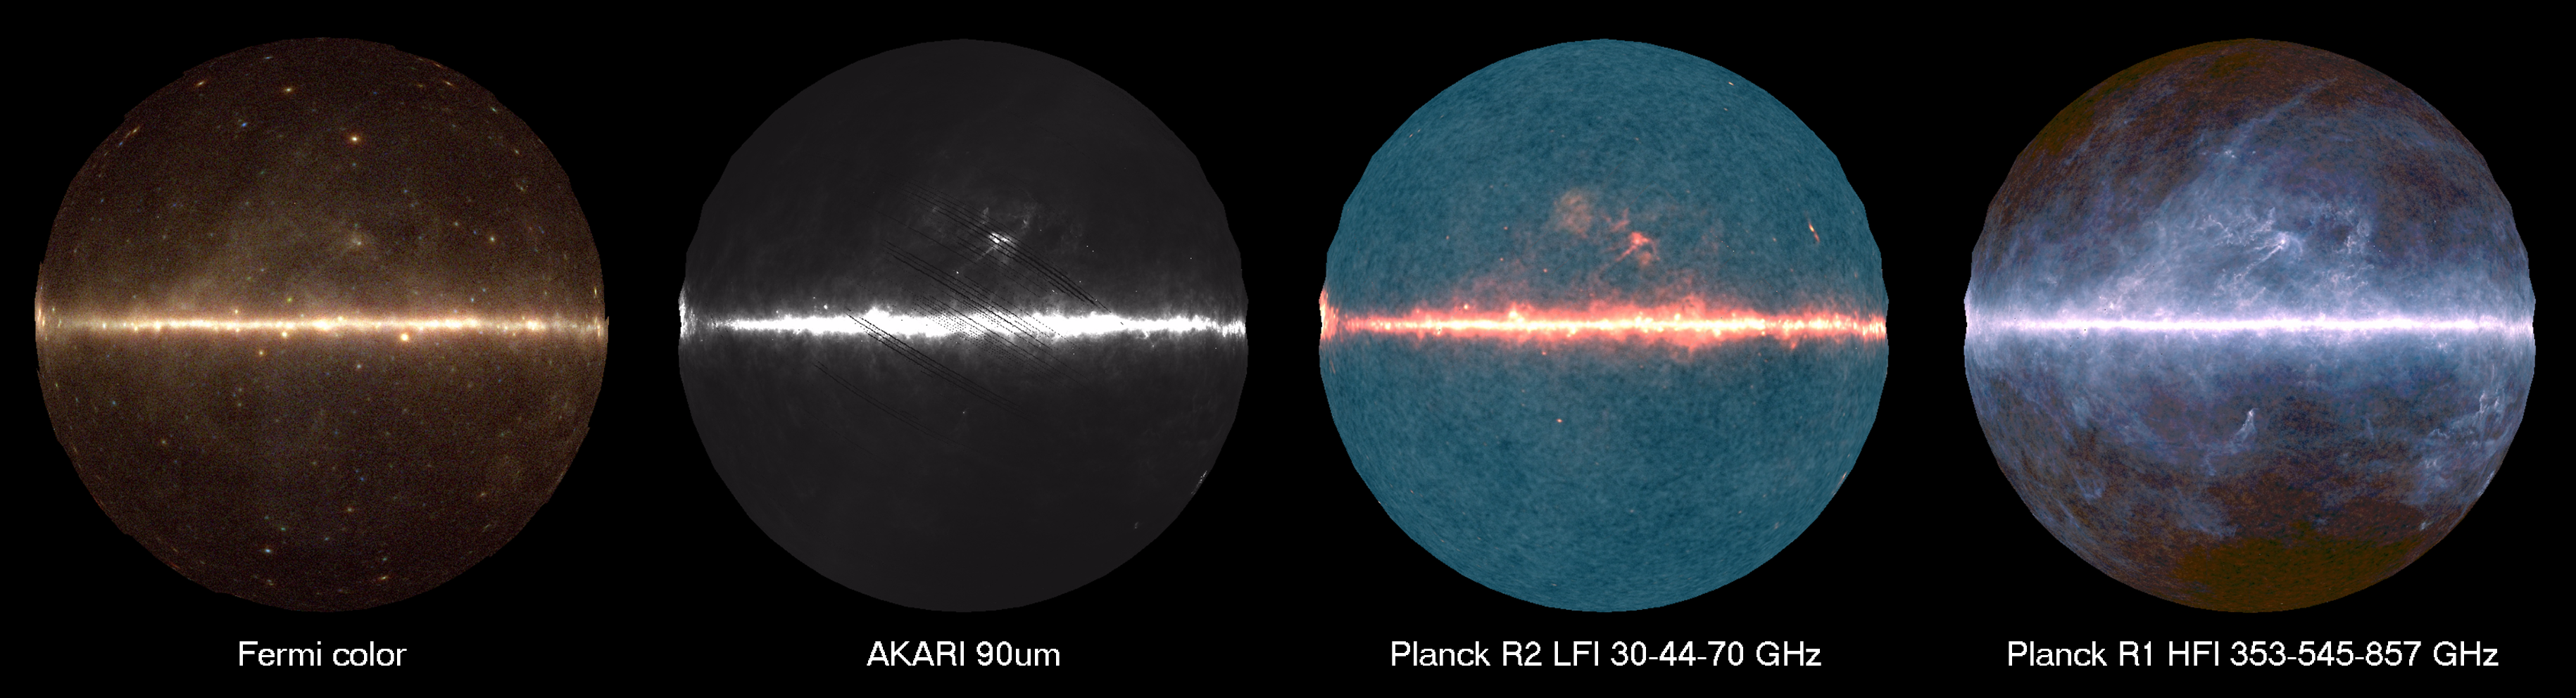
\includegraphics[width=\textwidth]{figures/four_images}}
  \caption{Survey images (left to right): Fermi color, AKARI 90um, Planck LFI, Planck HFI. Images centered on the Galactic Center, FOV 180 degrees.}
  \label{fig:four_images}
\end{figure}

% \begin{figure}[tb]
%   \centerline{\includegraphics[width=\textwidth]{figures/inner_galaxy_region}}
%   \caption{The inner galaxy in various survey images and color maps, FOV 45 degrees.}
% \end{figure}

% \begin{figure}[tb]
%   \centerline{\includegraphics[width=\textwidth]{figures/vela_region}}
%   \caption{The Vela Region in various survey images and color maps, FOV 20 degrees.}
%   \label{fig:vela_region}
% \end{figure}

\begin{figure}[tb]
  \centerline{\includegraphics[width=\textwidth]{figures/galactic_region_NEW}}
  \caption{The inner galaxy in various survey images and color maps, FOV $90 \times 15$ degrees. The red (TeV) and green (SNRcat) markers indicate many galactic SNRs and pulsars detected at very-high-energies.}
  \label{fig:galactic}
\end{figure}

\begin{figure}[tb]
  \centerline{\includegraphics[width=\textwidth]{figures/cygnus_region}}
  \caption{The Cygnus Region in various survey images and color maps, FOV $20 \times 10$ degrees. Sources of interest include: the diffuse emission nebula surrounding the Gamma Cygni star, the cosmic-ray Cygnus Cocoon observed by Fermi, and a handful of unidentified TeV sources indicated with red (TeV) markers.}
  \label{fig:cygnus}
\end{figure}
%
% \begin{figure}[tb]
%   \centerline{\includegraphics[width=\textwidth]{figures/lmc_region}}
%   \caption{The Large Magellanic Cloud (LMC) in various survey images and color maps, FOV 10 degrees.}
% \end{figure}

The default image layer displayed on the website's Map View page is a multi-wavelength all-sky survey from Fermi-LAT. As Fermi data is broken into multiple bands of energies, the map's native color scheme represents detected energies as categorized colors - red/yellow for the 0.3--1 GeV band, green for the 1--3 GeV band, and blue for the 3--300 GeV band.

 The Fermi color image is presented on the website as a Hierarchical Progressive Survey (HiPS) image \cite{hips}. HiPS is a hierarchical data structure utilizing the HEALPix\footnote[4]{\url{http://healpix.sourceforge.net/}} tesselation of a sphere that organizes data onto pixelated tiles of scalable resolution. The image mechanism allows catalog data and source markers on \gammasky to be visualized accurately on the sky map at various zoom levels. The Centre de Donn\'{e}es astronomiques de Strasbourg (CDS) developed the HiPS technology, and \gammasky currently encompasses 10 survey images also prepared by CDS in this format. The 10 images, which are outlined in Table~\ref{tab:images}, come from CDS's HiPS database\footnote[5]{\url{http://aladin.u-strasbg.fr/hips/list}} of over 300 prepared HiPS images. Four selected images are displayed on the three-dimensional sphere in Figure~\ref{fig:four_images}.

Our website incorporates 4 source catalogs, as illustrated in Table~\ref{tab:catalogs}. 3FGL \cite{3fgl} and 2FHL \cite{2fhl} are the latest source catalogs from Fermi-LAT, the main space-based instrument we display sources from. SNRcat \cite{snrcat} is an up-to-date compilation of galactic SNRs observed from a variety of instruments. The database is maintained by the University of Manitoba and can be accessed at \url{http://www.physics.umanitoba.ca/snr/SNRcat/}. gamma-cat is an open-data catalog of sources in the TeV range. As a project that has just recently begun in early September 2016, it is undergoing rapid growth and will be updated frequently on \gammasky. gamma-cat was started at the Max-Planck-Institut f\"{u}r Kernphysik (MPIK) and is open to contribution from other developers. All of its source information can be found at \url{https://gammapy.github.io/gamma-cat/}.

User inputs for search fields under the Map View portion of the website are interpreted by the Sesame service\footnote[6]{\url{http://cds.u-strasbg.fr/cgi-bin/Sesame}}. Sesame is a search term resolver for astronomical objects which queries several databases and returns the resolved sources. Both Sesame and the databases searched (SIMBAD, NED, and VizieR) are maintained by CDS.

Under the Catalog View of \gammasky, we are currently showing 3FGL light curve and emission spectrum plots from NASA's Fermi-LAT 3FGL Catalog Interactive Table\footnote[7]{\url{http://fermi.gsfc.nasa.gov/ssc/data/access/lat/4yr_catalog/3FGL-table}}.

\section{Implementation}

\begin{itemize}
\item Gammapy, Astropy used to generate catalog data (and map data)
\item Data consumed with JS and HTML
\item Website architecture built with Angular 2 as a single-page app
\item Sphere interface and maps overlay by Aladin Lite tool
\end{itemize}

\section{Status and Outlook}


Our website is a new project, having been deployed very recently at \url{http://gamma-sky.net} in early June 2016. The current content of \gammasky is simply a starting point; we have plans to greatly expand on our catalog and image data. Such data includes additional image surveys from CDS' HiPS database, as well as data from upcoming surveys upon their public release. The Fermi high-energy images are among the images we will prepare with HiPS for display on the Map View. We additionally strive to enhance the user interface of \gammasky through additional features, including new source groupings by classification as done in NASA's Fermi-LAT 3FGL Catalog Interactive Table\footnote[6]{\url{http://fermi.gsfc.nasa.gov/ssc/data/access/lat/4yr_catalog/3FGL-table}} and more intricate data panels for the Catalog View. Using Angular 2, an improved routing network will be implemented  to allow for sharing a specific view in the Map View page by URL. We will continue to point directly to Gammapy scripts for any further analysis and keep server-heavy tools off our website.

\section{Acknowledgements}

We would like to thank CDS (Centre de Donn\'{e}es astronomiques de Strasbourg) for developing the data formats (HiPS) and tools (Aladin Lite) that make \gammasky possible. Thomas~Boch helped us configure Aladin Lite to our use case. We would also like to thank: GitHub for hosting our website; CDS for serving the HiPS images; and all of the contributors to the open-source projects, including Angular 2, Astropy, and Gammapy, that we have used to build \gammasky.


% References

\nocite{*}
\bibliographystyle{aipnum-cp}
\bibliography{gammaskynet-gamma2016}

\end{document}
